\documentclass{standalone}

\usepackage{tikz}

\begin{document}

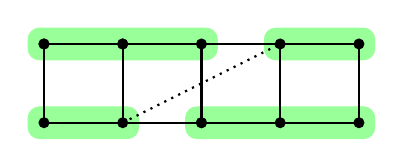
\begin{tikzpicture}

\filldraw[rounded corners, green!40!white] (-0.2,-0.2) rectangle (1.2,0.2);
\filldraw[rounded corners, green!40!white] (1.8,-0.2) rectangle (4.2,0.2);
\filldraw[rounded corners, green!40!white] (-0.2,0.8) rectangle (2.2,1.2);
\filldraw[rounded corners, green!40!white] (2.8,0.8) rectangle (4.2,1.2);

\node at (0,1) {}; 
\node  at (4,1) {}; 
\node  at (4,0) {}; 
\node at (0,0) {}; 
\node at (1,1) {};
\node at (2,1) {};
\node at (3,1) {};
\node at (1,0) {};
\node at (2,0) {};
\node at (3,0) {};

\foreach \i in {0,...,4}
{
    \fill (\i,0) circle (2pt);        
    \fill (\i,1) circle (2pt);        
    \draw[thick] (\i,0) -- (\i,1);
}
\foreach \i in {0,...,3}
{
    \draw[thick] (\i,0) -- (\i+1,0);
    \draw[thick] (\i,1) -- (\i+1,1);
}

    \fill (0,1) circle (2pt);
    \fill (1,1) circle (2pt);
    \fill (2,0) circle (2pt);

\draw[dotted, thick] (1,0) -- (3,1);

\end{tikzpicture}

\end{document}
